%\documentclass[12pt,compress,aspectratio=169]{beamer}
%\input{../mybeamer}
%
\chapter{Physical Optics}
%\subtitle{Unit 4: The Wave Nature of Light}
%\input{../term}
%\input{../mycommands}

\section{Double-Slit Interference}

The \textbf{double-slit experiment} was a demonstration that light behaves like
a wave. The experiment was conducted in 1801 by British physicist Thomas Young.
The experimental set-up is shown schematically in
Fig.~\ref{fig:double-slit-setup}.
\begin{figure}[ht]
  \centering
  \pic{.6}{physicalOptics/graphics/double-slit1}
  \caption{Thomas Young's double-slit experiment}
  \label{fig:double-slit-setup}
\end{figure}
Young first passed sunlight through a single slit\footnote{The general term
for any opening that allows light to pass through is a called an
\textbf{aperture}. In this case, a slit refers to a narrow rectangular
aperture.} . Two slits, arranged side by side, are equal distance to the single
slits. This creates two coherent (i.e.\ in phase) light sources. The light from
double-slit is then projected onto a screen. When the two slits are far apart,
two overlapping patches of light appeared on the screen, but when the slits
were brought closer together, the light created bands of colour separated by
dark regions. Young called these bands ``interference fringes''.

The double-slit experiment provided evidence that light was a wave, not a
particle, as Isaac Newton's corpuscular theory had proposed. However, Young's
work was criticized by most English scientists at the time.  The double-slit
experiment has since been used to demonstrate that other particles, like
electrons, can also behave like waves. The experiment has had a profound impact
on quantum physics, which now acknowledges that light and matter can exhibit
both wave and particle behaviour.
\begin{remark}
  Thomas Young's original experiment uses sunlight as a light source, which is
  \emph{broadband}, meaning that it contains all the frequencies and
  wavelengths within the visible-light spectrum. As we will see later in this
  chapter, this can cause the light to disperse into component waves when passed
  through the slits. Instead, more modern double-experiments use a
  \textbf{monochromatic light source}, which is a light containing a
  \emph{single} colour (frequency). This can be achieved with a laser,
  light-emitting diode (LED), or gas lamps with filters.
\end{remark}
The interference behaviour shown in the double-slit experiment is not unique to
light; the same behaviour are also shown in ocean waves and sound waves.

\begin{figure}[ht]
  \centering
  \begin{subfigure}[t]{.32\textwidth}
    \begin{tikzpicture}[scale=.3]
      % Slits
      \draw[slits] (0,1.1)--(0,3);
      \draw[slits] (0,.9)--(0,-.9);
      \draw[slits] (0,-1.1)--(0,-3);
      \node[left] at (-.1, 1){$S_1$};
      \node[left] at (-.1,-1){$S_2$};
      % Screen
      \draw[ultra thick,blue!60] (10,7)--(10,-7);
      % Centre line
      \draw (0,0)--(10,0);
      % Light waves
      \draw[functions,dash dot] (0,1)
      --(10,0) node[midway,above]{$L_1$}
      --(0,-1) node[midway,below]{$L_2$};
      \begin{scope}[functions,samples=80,domain=0:10]
        \draw[rotate around={-atan(.1):(10,0)}] plot(\x,{.4*sin(180*\x)});
        \draw[rotate around={ atan(.1):(10,0)}] plot(\x,{.4*sin(180*\x)});
      \end{scope}
      % Point P
      \fill (10,0) circle (.1) node[right]{\textbf{A} bright};
    \end{tikzpicture}
    \caption{At the centre line, $\Gamma=0$ and there is constructive
      interference.}
    \label{fig:point-A}
  \end{subfigure}
  \hspace{\stretch1}
  \begin{subfigure}[t]{.32\textwidth}
    \centering
    \begin{tikzpicture}[scale=.3]
      % Slits
      \draw[slits] (0,1.1)--(0,3);
      \draw[slits] (0,.9)--(0,-.9);
      \draw[slits] (0,-1.1)--(0,-3);
      \node[left] at (-.1, 1){$S_1$};
      \node[left] at (-.1,-1){$S_2$};
      % Screen
      \draw[ultra thick,blue!60] (10,7)--(10,-7);
      % Centre line
      \draw (0,0)--(10,0);
      % Light waves
      \draw[functions,dash dot] (0,1)--(10,-3) node[midway,above=3]{$L_1$}
      --(0,-1) node[midway,below=0]{$L_2$};
      \begin{scope}[functions,samples=80]
        \draw[domain=0:sqrt(116),rotate around={-atan(.4):(0,1)}]
        plot(\x,{.4*sin(167*\x)+1});
        \draw[domain=0:sqrt(104),rotate around={-atan(.2):(0,-1)}]
        plot(\x,{.4*sin(159*\x)-1});
      \end{scope}
      % Point P
      %\fill[gray] (10,0) circle (.1) node[right]{\textbf{A} bright};
      \foreach\y in {-3,3}
      \fill (10,\y) circle (.1) node[right]{\textbf{B} dark};
      %\fill (10,3) circle (.1) node[right]{\textbf{B} dark};
    \end{tikzpicture}
    \caption{At $B$, $\Gamma=\lambda/2$; there is total destructive
      interference.}
    \label{fig:point-B}
  \end{subfigure}
  \hspace{\stretch1}
  \begin{subfigure}[t]{.32\textwidth}
    \centering
    \begin{tikzpicture}[scale=.3]
      % Slits
      \draw[slits] (0,1.1)--(0,3);
      \draw[slits] (0,.9)--(0,-.9);
      \draw[slits] (0,-1.1)--(0,-3);
      \node[left] at (-.1, 1){$S_1$};
      \node[left] at (-.1,-1){$S_2$};
      % Screen
      \draw[ultra thick,blue!60] (10,7)--(10,-7);
      % Centre line
      \draw (0,0)--(10,0);
      % Light waves
      \draw[functions,dash dot] (0,1)--(10,-6) node[midway,above]{$L_1$}
      --(0,-1) node[midway,below]{$L_2$};
      \begin{scope}[functions,samples=80]
        \draw[domain=0:sqrt(149),
          rotate around={-atan(.7):(0,1)}] plot(\x,{.4*sin(177*\x)+1});
        \draw[domain=0:sqrt(125),
          rotate around={-atan(.5):(0,-1)}] plot(\x,{.4*sin(161*\x)-1});
      \end{scope}
      % Point P
      %\fill[gray] (10,3) circle (.1) node[right]{\textbf{B} dark};
      %\fill[gray] (10,0) circle (.1) node[right]{\textbf{A} bright};
      %\fill[gray] (10,-3) circle (.1) node[right]{\textbf{B} dark};
      \foreach \y in {-6,6}
      \fill (10,\y) circle (.1) node[right]{\textbf{C} bright};
      %\fill (10, 6) circle (.1) node[right]{\textbf{C} bright};
    \end{tikzpicture}
    \caption{At $C$, $\Gamma=\lambda$; there is constructive interference
      again.}
    \label{fig:point-C}
  \end{subfigure}
\end{figure}
To study the double-slit interference behaviour, we first define the
\textbf{path difference} $\Gamma$ to be the difference in distance to the two
slits where light emerge from:
\begin{equation}
  \Gamma=|L_1-L_2|
\end{equation}
\begin{itemize}[itemsep=6pt]
\item\textbf{Constructive interference at position A:} Along the centre line in
  Fig.~\ref{fig:point-A}, $\Gamma=0$ (i.e.\ $L_1=L_2$). If the light emitted
  from the slits are coherent (i.e.\ the two beams of light are in phase),
  there is constructive interference at \textbf{A}, and the projection is
  bright.

\item\textbf{Destructive interference at position B:} Further away from the
  centre line, on both sides of the centre line, shown in
  Fig.~\ref{fig:point-B}, the path difference is half of a wavelength:
  \begin{equation*}   
    \Gamma=|L_1-L_2|=\frac\lambda2
  \end{equation*}
  If light emitted from the two slits are coherent, they will arrive at
  \textbf{B} out of phase by \ang{180}. Therefore there is \emph{complete}
  destructive interference, and the projection is dark.
  
\item\textbf{Constructive interference at position C:} Still, further away from
  the centre line, on both sides of the centre, shown in
  Fig.~\ref{fig:point-C}, the path difference is exactly one wavelength:
  \begin{equation*}
    \Gamma=|L_1-L_2|=\lambda
  \end{equation*}
  If light emitted from the two slits are coherent, when the two beams of light
  arrive at \textbf{C}, they are once again in phase. Therefore, there is 
  constructive interference, and the projection is bright.
\end{itemize}

We can generalize the observations of various points along the screen. In the
most general form:
\begin{itemize}
\item If light emerging from the slits are coherent, a
  \textbf{constructive maximum} occurs when the path difference is a
  whole-number multiple of the wavelength:
  \begin{equation}
    \boxed{
      \Gamma_c = n\lambda
    }
  \end{equation}
\item Conversely, a \textbf{destructive minimum} occurs when the path
  difference is a half-number ($n+\frac12$) multiple of the wavelength:
  \begin{equation}
    \boxed{
      \Gamma_d = \left[n+\frac12\right]\lambda
    }
  \end{equation}
\end{itemize}
We will use the geometry of the double-slit problem to calculate $\Gamma$. The
end result is an alternating band of bright and dark ``fringes'' appearing on
the screen, as shown in Figure~\ref{fig:fringes}. The ``bright fringes'' are
the constructive maxima; the ``dark fringes'' are the destructive minima.
\begin{figure}[ht]
  \centering
  \pic{.35}{physicalOptics/graphics/fringes1}
  \caption{Bright and dark fringes appearing on the screen.}
  \label{fig:fringes}
\end{figure}



\subsection{Geometry of the Double-Slit Interference}
To better understand the basic behaviour of light in a double-slit experiment,
we construct a system shown in Figure~\ref{fig:basic-2-slit} (which is similar
to the earlier example).
\begin{figure}[ht]
  \centering
  \begin{tikzpicture}[scale=.65]
    % Draw the slits
    \draw[slits] (0,1.1)--(0,3);
    \draw[slits] (0,.9)--(0,-.9);
    \draw[slits] (0,-1.1)--(0,-3);
    \draw[|<->|] (-.5,-1)--(-.5,1) node[midway,left]{$d$};
    \node at (-.7,1.5) {$S_1$};
    \node at (-.7,-1.5) {$S_2$};
    % Draw the screen
    \draw[ultra thick,blue!60] (20,5)--(20,-2.5);
    % Draw dimension of the problem
    \draw[<->] (0,0)--(20,0) node[midway,fill=white]{$L$};
    \draw[|<->|] (20.7,0)--(20.7,3) node[midway,fill=white]{$y$};
    % Draw rays to P
    \draw[functions] (0,1)--(20,3)--(0,-1);
    \draw[dotted] (0,0)--(20,3);
    \draw[<->] (15,0) arc (0:atan(3/20):15)
    node[midway,right]{$\theta$};
    \fill (20,3) circle (.13) node[above right]{$P$};
  \end{tikzpicture}
  \caption{Geometry of a basic double-slit experiment}
  \label{fig:basic-2-slit}
\end{figure}
\begin{enumerate}[itemsep=4pt]%,leftmargin=15pt]
\item Two narrow slits  $S_1$ and $S_2$ of width $W$ are separate by a distance
  $d$. We assume that $d\gg W$, and therefore the light emerging from $S_1$ and
  $S_2$ can be treated as two \emph{coherent point sources}, i.e.\ two point
  sources that are in phase
\item A screen is located at a distance $L$ that is very far from the slits,
  i.e.\ $L\gg d$, and parallel to the slits
\item Light from $S_1$ and $S_2$ is projected onto the screen at location $P$,
  which is a lateral distance of $y$ away from the centre line. The lateral
  angle of deflection is $\theta$
\end{enumerate}
Fig.~\ref{fig:close-up1} shows a close-up of the slits.
%In this geometry, we make assumptions about the relative size of the different
%dimensions:
\begin{figure}[ht]
  \centering
  \begin{tikzpicture}[scale=.8]
    % Draw the slits
    \draw[slits] (0,1.05)--(0,3);
    \draw[slits] (0,.95)--(0,-.9);
    \draw[slits] (0,-1.05)--(0,-3);
    \draw[|<->|] (-.4,-1)--(-.4,1) node[midway,fill=white]{$d$};
    \node at (-.4,1.3) {$S_1$};
    \node at (-.4,-1.3) {$S_2$};
    \draw[dashed] (0,-1)--(5,-1);
    \draw[dashed] (0, 1)--(5, 1);
    \draw[vectors,red,rotate around={20:(0,-1)}](0,-1)--(5,-1);
    \begin{scope}[rotate around={20:(0,1)}]
      \draw[vectors,red] (0,1)--(5,1);
      \draw[dashed] (0,1)--(0,-1);
      \draw[|<->|] (0,-1.2)--(-.7,-1.2)
      node[midway,below right]{$\Gamma=d\sin\theta$};
      \draw[<-] (0,-.2) arc (270:250:1.2) node[midway,below]{$\theta$};
    \end{scope}
    \draw[->] (4.5,-1) arc (0:20:4.5) node[midway,right]{$\theta$};
    \draw[->] (4.5,1) arc (0:20:4.5) node[midway,right]{$\theta$};
  \end{tikzpicture}
  \caption{Close up view of the slits.}
  \label{fig:close-up1}
\end{figure}
When the screen is very far away from the slits, the two beams of light
arriving from the two slits at $P$ from the slits are \emph{approximately}
parallel. Using basic geometry, we can easily calculate the path difference
$\Gamma$ from the two slits to the screen:
\begin{equation}
  \Gamma=d\sin\theta
  \label{eq:path-difference-gamma}
\end{equation}
\begin{remark}
  Of course, the two beams of light are \emph{not} parallel, but the farther
  the screen is from the slits, the better the approximation
  Eq.~\ref{eq:path-difference-gamma} is. If the screen is, in fact, close to
  the slits, more sophisticated calculations will be needed to describe the
  interference pattern.
\end{remark}



\subsection{Constructive Maxima \& Destructive Minima}

A \textbf{constructive maximum}, or \textbf{anti-nodal point}, appear as a
\textbf{bright fringe} on the screen at lateral angle $\theta$ when the path
difference ($\Gamma=d\sin\theta$) is a whole-number ($n$) multiple of the
wavelength ($\lambda$):
\begin{equation}
  \boxed{
    d\sin\theta_n = n\lambda
  }
  \quad\text{where}\quad
  n=0,1,2\ldots,n_\text{max}
  \label{eq:2-slit-bright-fringe}
\end{equation}
The integer $n$ is called the \textbf{order number}\footnote{e.g.\ $n=0$ is
called the ``zeroth order''; $n=1$ is called ``first order'' etc}. The number
of bright fringes is not infinite. In Eq.~\ref{eq:2-slit-bright-fringe}, we
can see that the highest order fringe $n=n_\text{max}$ must occur when
$\sin\theta=1$:
\begin{equation}
  n_\text{max}=\left\lfloor\frac d\lambda\right\rfloor
\end{equation}
Since the fringes go from $-n_\text{max}\longrightarrow+n_\text{max}$, the
number of bright fringes $N$ is
\begin{equation}
  \boxed{
    N=2n_\text{max}+1=2\left\lfloor\frac d\lambda\right\rfloor+1
  }
  \label{eq:bright-fringes}
\end{equation}


Conversely, a \textbf{destructive minimum}, or \textbf{nodal point}), appear as
a \textbf{dark fringe} when $\Gamma$ is a half-number ($n+\frac12$) multiple of
the wavelength:
\begin{equation}
  \boxed{
    d\sin\theta_n = \left[n+\frac12\right]\lambda
  }
  \quad n=0,1,2\ldots
  \label{eq:dark-fringes}
\end{equation}




\subsection{Approximation of Wavelength}

The wavelength of light can be estimated based on the distance between fringes
using the \textbf{small-angle approximation}, where, for ``small angles''
measured in radians:
\begin{equation}
  \tan\theta\approx\sin\theta
\end{equation}
Using this approximation, we can replace the $\sin\theta$ in
Eq.s~\ref{eq:bright-fringes} (bright fringes) and
\ref{eq:dark-fringes} (dark fringes) with $\tan\theta$, which is also the
%We can approximate the $\sin\theta_n$ term with $\tan\theta_n$, which is the
ratio of the lateral distance of the $n$-th bright fringe ($y_n$) to the
distance to the screen ($L$):
\begin{equation*}
  n\lambda=
  %d{\color{red}\sin\theta_n}\approx
  d\tan\theta_n
  \quad\rightarrow\quad
  n\lambda\approx
  d\frac{y_n}L
\end{equation*}
%(As an exercise, compute $\tan\theta$ and $\sin\theta$ for $\theta=0.1$. For
%someone experienced in calculus, the approximation is obvious using Taylor
%series expansions of $\sin\theta$ and $\tan\theta$.)
Using this small-angle approximation, the lateral distance of the $n$-th bright
fringes from the centre anti-nodal line is given by:
\begin{equation} 
  \boxed{
    y_n\approx\frac{n\lambda L}d
  }
\end{equation}
And for the dark fringes, we can repeat the same approximation, but with $n$
replaced by $n+\frac12$:
\begin{equation}
  \boxed{
    y_n\approx\left[n+\frac12\right]\frac{\lambda L}d
  }
\end{equation}

In the region where small-angle approximation is valid, the lateral distance
to bright fringes is approximately \emph{linear} with $n$. In other words, for
the double-slit configuration, the bright fringes are evenly spaced. The
distance between the fringes is therefore:
\begin{equation*}
  \Delta y\approx\frac{\lambda L}d
\end{equation*}
Solving for wavelength $\lambda$, we have
\begin{equation}
  \boxed{\lambda\approx\frac{\Delta yd}L}
  \label{eq:wavelength-approximation}
\end{equation}




%{Approximation of Wavelength}
%The location of the $n$-th and $(n+1)$-th bright fringes are, respectively
%\begin{align*}
%  y_n&\approx\frac{n\lambda L}d\\
%  y_{n+1}&\approx\frac{(n+1)\lambda L}d
%\end{align*}
%Subtracting the two equations gives the expression for the approximate
%wavelength:

As the fringes are evenly spaced, Eq.~\ref{eq:wavelength-approximation}
applies equally to dark fringes as well as bright fringes.
\begin{common-question}
  \textbf{How small of an angle is small enough?} The origin of the small-angle
  approximation is based on the fact that leading terms in the series expansion
  of the $\sin\theta$ and $\tan\theta$ functions are both $\theta$ itself:
  \begin{align*}
    \sin\theta &=
    \theta-\frac{\theta^3}{3!}+\frac{\theta^5}{5!}-\frac{\theta^7}{7!}+\cdots\\
    \tan\theta &=
    \theta+\frac{\theta^3}3+\frac{2\theta^5}{15}+\frac{17\theta^7}{315}+\cdots
  \end{align*}
  (We have previously shown for the harmonic motion of the pendulum in
  Chapter~\ref{chapter:harmonic-motion} that we can approximate $\sin\theta$
  with $\theta$ for small angles.) As the angle increases, the two functions
  diverge quickly, but for small angles, there is good agreement. As is always
  the case, whether the angle is ``small enough'' depends on the numerical
  precision required in the calculations. We can calculate the error in this
  case using the equation
  \begin{equation*}
    \frac{\tan\theta-\sin\theta}{\sin\theta}\times\SI{100}\percent
  \end{equation*}
  To keep the error to less than \SI{10}{\percent} for two significant figures,
  the later angle should be kept to less \ang{20} from the centre line.
  \begin{center}
    \begin{tikzpicture}
      \begin{axis}[
          width=2.3in,
          xmin=0,xmax=3*pi/8,
          ymin=0,ymax=1.5,
          %xlabel=$\theta$ (radian),
          xtick={0,pi/8,pi/4,3*pi/8},
          xticklabels={0,$\dfrac\pi8$,$\dfrac\pi4$,$\dfrac{3\pi}8$},
          grid = both,
          legend pos=north west,
        ]
        \addplot[
          color=blue,
          domain=0:pi/2,
          samples=40,
          style={thick}]{sin(x*180/pi)};
        \addlegendentry{$\sin\theta$}
        \addplot[
          color=red,
          domain=0:3*pi/8,
          samples=40,
          style={thick}]{tan(x*180/pi)};
        \addlegendentry{$\tan\theta$}
        \addplot[
          color=orange,
          domain=0:pi/2,
          samples=40,
          style={thick}]{x};
        \addlegendentry{$\theta$}
      \end{axis}
    \end{tikzpicture}
    \hspace{\stretch1}
    \begin{tikzpicture}
      \begin{axis}[
          width=2.3in,
          ylabel=\% Error,
          xmin=0,xmax=3*pi/8,
          ymin=0,ymax=100,
          %xlabel=$\theta$ (radian),
          xtick={0,pi/8,pi/4,3*pi/8},
          xticklabels={0,$\dfrac\pi8$,$\dfrac\pi4$,$\dfrac{3\pi}8$},
          ytick={0,20,...,100},
          legend pos=north west,
          grid = both,
        ]
        \addplot[
          color=violet,
          domain=0:7*pi/16,
          samples=40,
          style=thick
        ]{abs(tan(x*180/pi)-sin(x*180/pi))/sin(x*180/pi)*100};
      \end{axis}
    \end{tikzpicture}
  \end{center}
\end{common-question}


There are several very important notes that we must make in studying the
double-slit problem:
\begin{enumerate}[itemsep=5pt]
\item The double-slit problem is applied specifically to visible light, but
  \emph{none} of the equation that were derived in this section are specific to
  visible light. We have chosen light because the constructive maxima and
  destructive minima (bright and dark fringes) are the easiest to discern for
  visible light. But if these equations points to a broader behaviour for
  waves, we must conclude they must also be applicable to \emph{any} wave,
  including mechanical waves like sound waves and ocean waves, but also other
  electromagnetic waves (radio waves, microwaves, infrared radiation,
  ultraviolet radiation, x-ray and gamma rays).

\item In formulating the equations the maxima and minima, we have effectively
  treated the slits as coherent point sources. In fact, it should be pointed
  out that replacing the slits with two actual coherent point sources will
  achieve a \emph{more accurate} result than two slits with physical width $W$,
  because a physical slit will cause diffraction, which is discussed in the
  next section.

\item The screen doesn't need to be a real screen either; it just
  has to be a location where wave amplitude can be measured. In fact, since
  all the equations came from calculating the path difference ($\Gamma$) from
  the two point sources, the ``screen'' does not even have to be parallel to
  the plane of the slits. Ultimately, the questions that must be asked,
  regardless of the geometry of the problem:
  \begin{center}
    \textbf{What is the path difference between the two point sources?\\
      How is the path difference related to the wavelength?}
  \end{center}
\end{enumerate}



\section{Single-Slit Diffraction}

When a wave goes through an small opening, it \textbf{diffracts}. This happens
with sound waves, ocean waves\ldots and light. For example,
Fig.~\ref{fig:alexandria} is an aerial photo of the Eastern Port in
Alexandria,Egypt. The shape of the entire harbour is created because of
diffraction of ocean wave.
\begin{figure}[ht]
  \centering
  \pic{.85}{physicalOptics/graphics/alexandria}
  \caption{Eastern Port in Alexandria}
  \label{fig:alexandria}
\end{figure}



%{Diffraction of Waves}
%  \begin{center}
%    \pic{.6}{graphics/diffraction1}
%  \end{center}
%  The smaller the opening (compared to the wavelength of the incoming wave)
%  the greater the diffraction effects.



\subsection{Geometry of the Single-Slit Diffraction}
The single-slit diffraction problem is similar to the double-slit problem:
\begin{figure}[ht]
  \centering
  \begin{tikzpicture}[scale=.65]
    % Draw the slits
    \draw[slits] (0,3)--(0,1);
    \draw[slits] (0,-3)--(0,-1);
    \draw[|<->|] (-0.5,-1)--(-0.5,1) node[midway,left]{$W$};
    % Draw the screen
    \draw[ultra thick,blue!60] (20,5)--(20,-3);
    % Draw dimension of the problem
    \draw[|<->] (0,0)--(20,0) node[midway,fill=white]{$L$};
    \draw[|<->|] (20.7,0)--(20.7,3) node[midway,fill=white]{$y$};
    % Draw rays to P
    \draw[functions] (0,1)--(20,3)--(0,-1);
    \draw[dotted] (0,0)--(20,3);
    \draw[<->] (15,0) arc (0:atan(3/20):15) node[midway,right]{$\theta$};
    \fill (20,3) circle (.13) node[above right]{$P$};
  \end{tikzpicture}
  \caption{Geometry of the basic single-slit diffraction problem}
  \label{fig:basic-1-slit}
\end{figure}
\begin{itemize}
\item A single slit of width $W$ instead of two slits. The width of the slit
  is small compared to the distance to the screen, but not insignificant
\item A screen located at a distance $L$ very far from the slit (i.e.\
  $L\gg W$), and parallel to it
\item Light from the top and bottom edges of the slit is projected at $P$
\end{itemize}



\subsection{Central Diffraction Maximum}
\begin{figure}[ht]
  \centering
  \begin{tikzpicture}[scale=1.3]
    \draw[slits] (0,2)--(0,1);
    \draw[slits] (0,-2)--(0,-1);
    \draw[|<->|,thick] (-.4,-1)--(-.4,1) node[midway,fill=white]{$W$};

    \foreach \y in {1,3,...,13} {
      \pgfmathsetmacro\yy{1.05-.15*\y}
      \draw[vectors,red] (0,\yy)--(4,\yy);
    }
    
    \foreach \y in {1,...,13} {
      \pgfmathsetmacro\yy{1.05-.15*\y}
      \fill (0,\yy) circle (.05);
    }
  \end{tikzpicture}
  \caption{Central diffraction maximum occurs at zero lateral angle}
  \label{fig:central-max}
\end{figure}
\begin{itemize}
\item Apply Huygens' principle, similar to the double-slit problem
\item The slit is wide enough that there is an infinite series
  of wavelets originating at the slit
\item Light from the wavelets that travel perpendicular to the slit
  interfere \emph{constructively}
\item A bright fringe at the middle, called the
  \textbf{central diffraction maximum}
\end{itemize}




\subsection{High-Order Maxima and Minima}

To locate the \textbf{destructive minima} (complete destructive interference,
appearing as dark fringes), we calculate the path difference between the upper
and lower edges, which is
\begin{equation*}
  \Gamma=W\sin\theta
\end{equation*}
where $\theta$ is the lateral angle measured from the optical centre line,
as shown in Fig~\ref{fig:single-slit-path difference}. The dots in the figure
are labelled 1 to 10 for convenience to represent the wavelets. There are,
of course, infinite number of these wavelets. This is similar to the analysis
for the double-slit.
\begin{figure}[ht]
  \centering
  \begin{tikzpicture}[scale=1.3]
    \draw[slits] (0,2.5)--(0,1);
    \draw[slits] (0,-1.7)--(0,-1);
    \draw[|<->|,thick] (-.4,-1)--(-.4,1) node[midway,fill=white]{$W$};

    \foreach \y in {1,6,10} {
      \pgfmathsetmacro \yy{1.1-.2*\y}
      \draw[vectors,red,rotate around={25:(0,\yy)}] (0,\yy)--(4,\yy);
    }

    \foreach \y in {1,...,10} {
      \pgfmathsetmacro \yy{1.1-.2*\y}
      \fill (0,\yy) circle (.05) node[left]{\sffamily\tiny$\y$};
    }
    \begin{scope}[rotate around={25:(0,.9)},dashed]
      \draw (0,.9)--(0,-1.3);
      \draw (-.76,-.76)--(-.76,-1.3);
      \draw[<->,thick] (-.76,-1.2)--(0,-1.2)
      node[midway,below right]{$\Gamma=W\sin\theta$};
    \end{scope}
    \draw[dashed] (0,-.9)--+(3.7,0);
    \draw[->] (3.5,-.9) arc(0:25:3.5) node[midway,right]{$\theta$};
  \end{tikzpicture}
  \caption{Path difference between edges for the single-slit}
  \label{fig:single-slit-path difference}
\end{figure}

At some lateral angle $\theta$, the path difference between wavelets 1 and 10
is one wavelength, i.e.\ $\Gamma=\lambda$. At this point, the path difference
between wavelets 1 and 6 is half a wavelength and the two waves cancel each
other completely. Likewise, wavelet 2 and 7 cancel, and wavelet 3 and 8 cancel,
etc. The result is that there is complete destructive interference. The same
destructive interference occurs again at lateral angle $\theta_2$ when the path
difference is wavelengths long, i.e. $\Gamma=2\lambda$.

Therefore, we can generalize the locations of the dark fringes---which represent
\emph{complete} destructive interference---to be when the path difference
($W\sin\theta$) is a whole-number ($m$) multiple of the wavelength ($\lambda$):
\begin{equation}
  \boxed{    
    W\sin\theta_m = m\lambda
  }
  \quad\text{where}\quad m=1,2,3\ldots
  \label{eq:1-slit-dark-fringe}
\end{equation}
Note that the indexing does not include $m=0$ because that is the location of
the central diffraction maximum.

We can also applying the small-angle approximation (approximating the
$\sin\theta_m$ term in Eq.~\ref{eq:1-slit-dark-fringe} with
$\tan\theta_m=y_m/L$) to relate the location of the dark fringes to the
corresponding lateral distance from the optical centre line:
\begin{equation}
  \boxed{y_m\approx\frac{m\lambda L}W}
\end{equation}


%{At Some Other Angle $\theta$}
%\begin{figure}[ht]
%  \centering
%  \begin{tikzpicture}
%    \draw[slits] (0,3)--(0,1);
%    \draw[slits] (0,-2)--(0,-1);
%    \draw[|<->|] (-.5,-1)--(-.5,1) node[midway,fill=white]{$W$};
%    \foreach \y in {1,...,13} {
%      \pgfmathsetmacro \yy{1.05-.15*\y}
%      \fill (0,\yy) circle (.03) node[left]{\tiny\y};
%    }
%    \foreach \y in {1,5,9,13} {
%      \pgfmathsetmacro \yy{1.05-.15*\y}
%      \draw[vectors,red,rotate around={30:(0,\yy)}] (0,\yy)--(5.5,\yy);
%    }
%    \begin{scope}[rotate around={30:(0,.9)},thick,dashed]
%      %\draw (0,.88)--(0,-.66);
%      \draw (0,-.66)--(-.9,-.66) node[pos=.9,right]{$W\sin\theta$};
%    \end{scope}
%  \end{tikzpicture}
%\end{figure}
%\begin{itemize}
%\item 
%\item Beam from (1) and (5) differ by $\dfrac\lambda2$, so they have
%  destructive interference; similarly 2 and 6, 3 and 7, 4 and 8, 9 and 13
%  will all interfere destructively
%\item But some of the beams will not, so we have a ``bright fringe'' at the 
%  projection
%\item 
%\end{itemize}
  

\textbf{Diffraction maxima} on either side of the central diffraction maximum
are located between the minima. Following the procedure for the diffraction
minima, we note that for some lateral angle $\theta_1$ when the path difference
between the top and bottom is one-and-a-half times the wavelength, i.e.\
$\Gamma=\frac32\lambda$, light emerging from the wavelets cannot completely
cancel, and therefore there would be a ``bright'' fringe appearing on the
screen. This bright fringe is not as bright as the central one because it is
the result of \emph{partial} destructive interference. We see again an even
dimmer ``bright'' fringe at $\theta_2$ when $\Gamma=\frac52\lambda$. Therefore,
we can generalize that these high-order maxima (bright fringes resulting from
partial destructive interference) exist on the screen at regular, half-number
($m+\frac12$) intervals:
\begin{equation}
  \boxed{
    W\sin\theta_m = \left[m+\frac12\right]\lambda
  }
  \quad\text{where}\quad m=1,2,3\ldots
\end{equation}
Again, the indexing starts at $m=1$ and not 0.

Similar to the dark fringes, the small-angle approximation gives this
equation:
\begin{equation}
  \boxed{y_m\approx\left[m+\frac12\right]\frac{\lambda L}W}
\end{equation}

\begin{remark}
  This equations for the single-slit diffraction look very similar to the
  equations for the double-slit interference. Be \emph{very} careful when you
  use them!
\end{remark}

\begin{example}
  Viewing a \SI{645}{\nano\metre} red light through a narrow slit cut into a
  piece of paper yields a series of bright and dark fringes. You estimate that
  five bright fringes appear in a space of \SI{5.0}{\milli\metre}. If the paper
  is \SI{32}{\centi\metre} from your eye, calculate the width of the slit.
\end{example}






%{Single-Slit Diffraction, A Summary}
\begin{itemize}
\item The single-slit diffraction projects a series of alternating bright
  fringes (``maxima'') and dark fringes (``minima'') onto the screen
\item The bright fringe in the middle (central diffraction maximum) is
  twice as wide and very bright
\item Subsequent bright fringes on either side (called
  \textbf{high-order maxima}) are
  much dimmer because of the partial destructive interference
\end{itemize}
\begin{center}
  \pic{.5}{physicalOptics/graphics/Single_Slit_Diffraction}
\end{center}



\section{Multiple-Slit Interference: Diffraction Grating}
Diffraction grating is when there are more than two slits. One such example is
shown in Fig.~\ref{fig:3-slit} for a three-slit configuration.
\begin{figure}[ht]
  \centering
  \begin{tikzpicture}[scale=.6]
    % Draw the slits
    \draw[slits] (0,1.1)--(0,3);
    \draw[slits] (0,.9)--(0,-.9);
    \draw[slits] (0,-1.1)--(0,-3);
    \draw[|<->|] (-.5,-1)--(-.5,1) node[midway,left]{$d$};
    \node at (-.7,1.5) {$S_1$};
    \node at (-.7,-1.5) {$S_2$};
    % Draw the screen
    \draw[ultra thick,blue!60] (20,5)--(20,-2.5);
    % Draw dimension of the problem
    \draw[<->] (0,0)--(20,0) node[midway,fill=white]{$L$};
    \draw[|<->|] (20.7,0)--(20.7,3) node[midway,fill=white]{$y$};
    % Draw rays to P
    \draw[functions] (0,1)--(20,3)--(0,-1);
    \draw[dotted] (0,0)--(20,3);
    \draw[<->] (15,0) arc (0:atan(3/20):15)
    node[midway,right]{$\theta$};
    \fill (20,3) circle (.13) node[above right]{$P$};
  \end{tikzpicture}
  
  \textbf{THIS IS THE WRONG DIAGRAM AT THIS MOMENT!}
  \caption{Geometry of a five-slit configuration}
  \label{fig:3-slit}
\end{figure}
A practical diffraction grating would have thousands of slits per centimetre.
Not surprisingly, diffraction gratings also show alternating bright and dark
fringes, although the analysis is slightly more complicated. We continue to
make the same assumptions from the analysis of the double slit.

Constructive maxima, where each slit interfere constructively with each other,
would still occur when the path difference between each of slits to the screen
are whole-number multiples of the wavelength. This means that the conditions
for constructive maxima are the same as for the double-slit configuration:
\begin{equation}
  d\sin\theta=n\lambda
  \label{grating-max}
\end{equation}
For the diffraction grating, the maxima specified in Eq.~\ref{grating-max} are
called \emph{primary} maxima. As we will see later, between primary maxima,
there are also secondary maxima.

Locating the destructive minima is somewhat more complicated. Take the
three-slit configuration in Fig.~\ref{fig:3-slit} as an example, \emph{complete}
destructive interference would occur when the path difference between the slits
is
\begin{equation*}
  \Gamma=\frac\lambda3, \frac{2\lambda}3,
  \frac{4\lambda}3, \frac{5\lambda}3,\ldots
\end{equation*}
This is shown graphically in Fig.~\ref{fig:grating-destructive}.
\begin{figure}[ht]
  \centering
  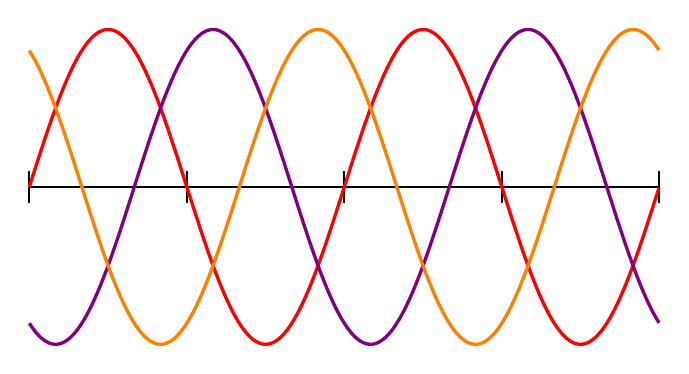
\begin{tikzpicture}[scale=2]
    \draw[thick] (0,0)--(4,0);
    \foreach\x in {0,1,2,3,4} \draw[thick] (\x,.1)--(\x,-.1);
    \begin{scope}[very thick,domain=0:4,samples=100,smooth]
      \draw[red] plot(\x,{sin(180*\x)});
      \draw[violet] plot(\x,{sin(180*\x-120)});
      \draw[orange] plot(\x,{sin(180*\x-240)});
    \end{scope}
  \end{tikzpicture}
  \caption{Path difference with total destructive interference. The sum of the
  three waves out of phase by $\lambda/3$ is zero.}
  \label{fig:grating-destructive}
\end{figure}

We can generalize this for any diffraction with $N$ slits, destructive minima
occur at
\begin{equation}
  d\sin\theta=
  \left(n+\frac mN\right)\lambda
  \quad\text{where}\quad n=0,1,2,\ldots \text{ and }m=1,...,N-1
  \label{grating-min}
\end{equation}
In between the destructive minima are the secondary maxima where there is
partial destructive interference. The brightness (wave intensity) of the
secondary maxima are much lower than the primary, and are not always visible.
Therefore the visible interference pattern for the diffraction grating is much
sharper than the two-slit pattern, and the bright fringes (primary maxima) are
also narrower.


\begin{figure}[ht]
  \centering
  \pic{.5}{physicalOptics/graphics/grating1}
\end{figure}

\section{Optical Resolution}
The ability of an optical instrument (e.g.\ the human eye, microscope,
camera) to distinguish two distinct objects.
\begin{figure}[ht]
  \pic{.3}{physicalOptics/graphics/resolve1}
  \pic{.3}{physicalOptics/graphics/resolve2}
  \pic{.3}{physicalOptics/graphics/resolve3}
\end{figure}
When light from any object passes through any optical instrument, it
\emph{diffracts}, therefore ``blurring'' the object.




%  
%    \pic1{graphics/resolve4}

In the \textbf{Rayleigh criterion}, two objects are resolved if the angle
$\theta>\theta_\text{min}$, where $\theta_\text{min}$ is when the first
minimum (dark fringe) from object 1 overlaps with the central maximum
(bright fringe in the middle) from object 2.

To resolve two objects, the minimum angle of separation $\theta_\text{min}$
between rays from the two object passing through an aperture depends on the
shape of the aperture. For a rectangular aperture:
\begin{equation}
  \boxed{\theta_\text{min}=\frac\lambda W}
\end{equation}
where $\lambda$ is the wavelength of light passing through, and $W$ is the
width of the aperture. For a circular aperture:
\begin{equation}
  \boxed{\theta_\text{min}=\frac{1.22\lambda}D}
\end{equation}
where $D$ is the
diameter of the aperture.

Note that the angle $\theta_\text{min}$ is measured in \emph{radians} not
degrees.

\begin{example}
  A skydiver is falling towards the ground. How close to the ground will she
  have to be before she is able to distinguish two red balls lying
  \SI{25.0}{\centi\metre} apart, reflecting \SI{625}{\nano\metre} light in air?
  Her pupil diameter is \SI{3.35}{\milli\metre}. Assume that the speed of
  light inside the human eye is \SI{2.21e8}{\metre\per\second}.
\end{example}



\section{Angular Dispersion of Light by Diffraction}
The examples for single- and double-slit patterns that have all been based on
a \emph{single} wavelength of light, but we know that the equations depends on
wavelength. So what happens to our diffraction pattern when the light source
is a white light?
\begin{figure}[ht]
  \centering
  \pic{.7}{physicalOptics/graphics/57010}
  \caption{Interference pattern for white light}
\end{figure}

